\chapter{Bitcoin Blockchain}
The following chapter will show how the Bitcoin blockchain works and that it has the following properties.

\begin{center}
	\begin{tabular}{|c c c|} 
     \hline
     Problem & Solved & Not Solved \\ [0.5ex] 
     \hline
     Decentralization & \checkmark  & \\ [0.5ex] 
     \hline
     Privacy & \checkmark &  \\ [0.5ex] 
     \hline
     Double-spending & \checkmark  & \\ [0.5ex] 
     \hline
     Byzantine generals problem & \checkmark  & \\ [0.5ex] 
     \hline
     Backed by energy & \checkmark & \\ [0.5ex] 
     \hline
     Sybil attacks & \checkmark &  \\ [0.5ex]
     \hline
     Inflation resistant & \checkmark & \\ [0.5ex] 
     \hline
    \end{tabular}
\end{center}


\section{Peer to Peer Network}

Most pioneer concepts described in this thesis either relied on a trusted third party or were never implemented due to their susceptibility to double-spending, inflation, Sybil attacks, or the lack of byzantine fault tolerance.
The Bitcoin core protocol is designed as a peer-to-peer network. 
Every computer running the software acts as a node.
However, a node can act as an active or passive network node.
Active nodes are identifiable by their public IP address, while private ones use their local IP address to connect to the network.
This results in public nodes acting as peers accepting incoming connections from around the globe.

In the following, the term peers will reference publicly available nodes, while the term node references a network node inaccessible over the internet.
Both peers and nodes can maintain eight outgoing connections at the same time.
In addition, a peer accepts up to 117 incoming connections.

If a new node or peer is to join the network, a bootstrapping protocol is used to connect it to other peers.
The protocol uses a domain name server to acquire a list of active peers. 
Otherwise, it connects to hardcoded addresses.
After successfully connecting to a peer, it receives even more addresses to establish more connections.
In addition, the peer also sends all verified transactions and blocks.
The new participant verifies and accepts the data according to the network consensus rules programmed into its software. \cite{Zaghloul2020}
\begin{center}
	\begin{tabular}{|c c c|} 
     \hline
     Problem & Solved & Not Solved \\ [0.5ex] 
     \hline
     Decentralization & \checkmark  & \\ [0.5ex] 
     \hline
    \end{tabular}
\end{center}

\section{Digital coins}

Former implementations of digital cash, like Chaum's ecash, used databases with accounts to track every user's balance.
Satoshi chose a different approach, called \textbf{Unspent Transaction Outputs} (UTXO).
This idea is very similar to Finney's concept of tracking the chain of ownership of RPOW tokens.
Instead of units of Bitcoin just being a number in a database, they are tracked in UTXOs.
They act like digital cash with a static value comparable to a dollar bill with a particular value.

Every user controls a Bitcoin wallet with a cryptographic keypair. 
The public key serves as a pseudonym for privacy purposes and is used to derive a wallet address.

\begin{center}
    \begin{tabular}{|c c c|} 
     \hline
     Problem & Solved & Not Solved \\ [0.5ex] 
     \hline
     Privacy & \checkmark  & \\ [0.5ex] 
     \hline
    \end{tabular}
\end{center}

A money transfer requires the creation of a hash using its latest transaction and the public key of the next owner.
This hash is then cryptographically signed by the sender with their private key, thus making the transfer verifiable with their public key.

Similar to Szabo's bit gold, a chain of verifiable ownership is formed.
Consequently, a Bitcoin wallet has access to UTXOs with different values.
However, one transaction does not only consist of one UTXO. 
Instead, it has multiple inputs and outputs.

\begin{figure}[htpb]
    \centering
    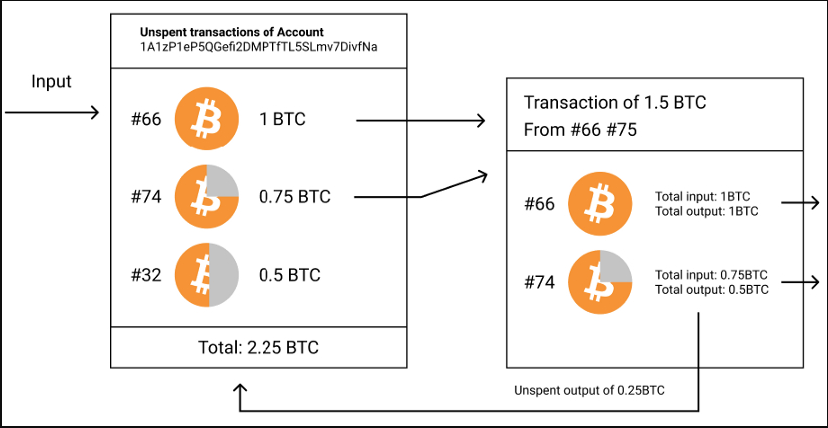
\includegraphics[width=\textwidth,height=6cm,keepaspectratio=true]{utxo_graphic_1.png}
    \caption{
        Sketch of the UTXO transaction format \cite{utxo_graphic1}
    }
\end{figure}

Consider a scenario with three users named Alice, Bob, and Greg.
Greg owns two UTXOs, each valued at 1 Bitcoin.
In total, he owns two bitcoins.
If he wants to send 1.2 bitcoins to Alice and 0.3 to Bob, he puts his two UTXOs into the input field of a newly created transaction.
The input field is already valid since he wants to spend less than he owns.
In addition, Greg must create two new UTXOs in the output field of the transaction to send the money to Alice and Bob.
The first new UTXO contains Alice's public key and the amount of 1.2 bitcoins.
The second new UTXO contains Bob's public key and the amount of 0.3 bitcoins.
Consequently, Greg creates a third UTXO referencing his wallet to receive the remaining value of 0.4 bitcoins as a change, leaving 0.1 bitcoin as a payment fee.

Nevertheless, Satoshi faced a significant problem referenced in his whitepaper.
How could a payee verify that the owner did not spend their coins in an earlier transaction?
This double-spending problem resulted in the need for a mechanism to reach a consensus among all network participants.
The solution had to be cryptographically verifiable and resilient to Sybil attacks or the byzantine fault tolerance problem.
Hence, Satoshi envisioned a distributed timestamping server that kept track of all transactions ever made.
These transactions are collected in so-called blocks.
Each block is a list of transactions. 
Every transaction has a list of input and output UTXOs.
Besides, a block has a timestamped block hash to save the block confirmation date.
Accordingly, all transactions inside a particular block are considered to have happened simultaneously.
Ultimately, a chain of blocks is formed by using the previous block hash as input for the next block hash.
This system is called blockchain and serves as a decentralized solution to the double-spending problem. 

\begin{center}
    \begin{tabular}{|c c c|} 
     \hline
     Problem & Solved & Not Solved \\ [0.5ex] 
     \hline
     Double-spending & \checkmark  & \\ [0.5ex] 
     \hline
    \end{tabular}
\end{center}

\section{Storage management}

Since every new block results in more storage space taken by the software, the constant growth of the blockchain must be limited.
That is why new blocks are created every ten minutes. \cite{nakamoto2008}
Using such a period also ensures the network has enough time to spread a newly found block to all network nodes until the next block is found.

Every block in the chain has a block header that is 80 bytes in size.
It contains the following parts.

\begin{center}
    \begin{tabular}{|c c|} 
     \hline
     Size & Name \\ [0.5ex] 
     \hline
     4 Bytes & Version \\ [0.5ex] 
     \hline
     32 Bytes & Previous block hash \\ [0.5ex] 
     \hline
     32 Bytes & Merkle root hash \\ [0.5ex] 
     \hline
     4 Bytes & Timestamp \\ [0.5ex] 
     \hline
     4 Bytes & nBits \\ [0.5ex] 
     \hline
     4 Bytes & Nonce \\ [0.5ex] 
     \hline
    \end{tabular}
\end{center}

The first four bytes represent the block version. This allows future soft forks to upgrade the block validation rules over time.
Next to them are 32 bytes that contain the previous block hash to ensure the immutability of the chain. This hash is built with the SHA256 algorithm.
A Merkle tree is built to save the transactions inside a block from manipulation. The root of the Merkle tree can be used to validate a particular transaction.
It is 32 bytes in size and also a part of a block header.
The next four bytes are used to store the timestamp, followed by four bytes for the mining difficulty target and four bytes for the mining nonce. \cite{blockheaders}
Mining will be discussed in the Proof of Work chapter of this thesis.

In addition, the number of transactions per block is limited due to a maximum size of one megabyte per block \cite{8215367}.
This results in a maximum potential blockchain growth of:

\begin{equation}
    1MB * 6 * 24 * 365 = 52,560MB = 52.560GB.\textrm{ per year}
\end{equation}

The slow storage increase ensures that running a Bitcoin full node is affordable for everyone, leading to more potential peers on the network. \cite{nakamoto2008}
Consequently, even if a central authority owned thousands of nodes, it would still be unable to control the network because users could still build a node and choose the consensus rules themselves.
Accordingly, when new versions of the software are published, every user who owns a node decides on their own whether to install it.
A new version of the code that would change consensus rules and break compatibility would have to be accepted by nearly every user who runs a node to become a reality in the network. 
This procedure solves the byzantine fault tolerance problem, as every node can verify the transactions independently.
The information is only spread if it is validated. Otherwise, it will be discarded.
\begin{center}
    \begin{tabular}{|c c c|} 
     \hline
     Problem & Solved & Not Solved \\ [0.5ex] 
     \hline
     Byzantine generals problem & \checkmark  & \\ [0.5ex]
     \hline
    \end{tabular}
\end{center}

\section{Proof of Work Consensus}

Reaching consensus in a peer-to-peer network is a challenging problem.
Since the network is freely usable, it must be resilient against bad actors.
Whenever a new block is needed to validate transactions and reach a new network state, someone has to select transactions for the next block and find a valid hash.
Therefore, if a bad actor were to create all upcoming blocks, he could censor specific wallets by excluding their transactions forever.
If it were predetermined who gets to validate the next block, it would leave room for corruption or censorship.
Therefore, the next person to validate a block must be randomly selected.
Satoshi used Adam Backs Hashcash to implement a Proof of Work consensus algorithm to achieve that. 
Each block hash needs to meet specific requirements to be accepted by the network.
Like Hashcash, a miner needs to find a nonce so that the block hash is smaller than a particular target.
The target is chosen by the network and adjusted after every period of 2014 valid blocks.
The adjustment ensures blocks are found every ten minutes on average by raising or lowering the required target for a valid hash.
This process is called difficulty adjustment.

Every miner has a certain probability of finding a valid hash for the block header. 
The more computing power the miner has, the more likely they will be the first to find a valid hash. 
Nevertheless, miners with lower hash rates also have a statistical chance of validating a block. 
If one miner controls 20 percent of the network's hash rate, their chance of finding a valid hash and receiving the block reward is also 20 percent.
This process is comparable to a lottery, where the contributed hash rate is a lottery ticket.
The higher the hash rate, the more lottery tickets.
As a result, it is random who gets to verify the next block based on their hash rate contribution.
However, whenever a new miner joins the network, the percentage of the total network's computing power changes.
Theoretically, a miner that controls at least 50 percent of the network's total hash rate could partially control the mining process by validating more blocks than any other miner.
Consequently, he could censor particular wallets or transactions.
Ultimately, even if any miner reaches this state, they must preserve their power by accumulating more hashing power as the network grows with new miners joining.

Using this technique solved a problem former electronic cash systems faced: the guaranteed inflation of digital money resulting from technological progress and faster computers in the future.
Still, that is not its only purpose.
Satoshi described Proof of Work as one-CPU-one-vote \cite{nakamoto2008}. 
The more leading zero bits it has, the more hashing power it takes to find the hash.
In addition, the block's timestamp further proves how long it took to find it.
Thus, A block's hash proves the global accumulated energy used to validate it because creating the hash took time and consumed energy.

\begin{center}
    \begin{tabular}{|c c c|} 
     \hline
     Problem & Solved & Not Solved \\ [0.5ex] 
     \hline
     Backed by energy & \checkmark & \\ [0.5ex] 
     \hline
    \end{tabular}
\end{center}

If a new computer is to enter the network, it needs to receive the chain from other peers.
Without Proof of Work, malicious peers could create fake chains and send them to new nodes.
Only the network difficulty and the block hash provide information that makes identifying the honest chain possible.
The chain with the greatest difficulty and, thus, the highest computational effort is most likely the honest chain \cite{nakamoto2008}.

In theory, creating a fake chain is only possible if one has more hashing power than the honest part of the network.
First, an attacker would have to recalculate all blocks that happened since the block they want to fake.
Then, they must calculate new blocks faster than the rest of the network to convince the network nodes that the fake chain is the honest chain.
If two chains exist in parallel, every network node will choose the faster-growing chain with the same difficulty and discard the other.
Thus, a central authority could only take over the consensus algorithm if it had more energy and hardware in control than the rest.
The Sybil attack is prevented by making it uneconomical and difficult to perform a system takeover.
\begin{center}
    \begin{tabular}{|c c c|} 
     \hline
     Problem & Solved & Not Solved \\ [0.5ex] 
     \hline
     Sybil attacks & \checkmark  & \\ [0.5ex]
     \hline
    \end{tabular}
\end{center}

Furthermore, the chain uses the Proof of Work consensus mechanism to issue new coins into the ecosystem.
Whenever miners find a valid block hash, they receive a transaction that pays a so-called block reward consisting of newly created coins and transaction fees.
In turn, miners are incentivized to secure the network with their hashing power, while the amount of new coins rewarded is halved every 210,000 blocks to prevent money supply inflation.
As a result, there is an upper supply limit of nearly 21 million bitcoins.
Bitcoin uses Proof of Work to solve the double-spending problem and to issue new coins into the system without the risk of hyperinflation or a central authority controlling the supply \cite{wirdum_2_2018}. 


\begin{center}
    \begin{tabular}{|c c c|} 
     \hline
     Problem & Solved & Not Solved \\ [0.5ex] 
     \hline
     Inflation resistant & \checkmark & \\ [0.5ex] 
     \hline
    \end{tabular}
\end{center}
\newpage
\section{Nodes}

Bitcoin is a peer-to-peer network consisting of computer nodes running the Bitcoin program.
There are four different types of node programs in total that serve different purposes.

\begin{itemize}
    \item Full node
    \item Header-only node
    \item Signing only (Wallet)
    \item Mining nodes
\end{itemize}

\textbf{Full nodes} run the original Bitcoin software. 
Thus, they include all protocol functionalities and keep a full copy of the blockchain.
Their main task is to verify incoming transactions or newly found blocks from the miners. 
If a block is valid, they propagate it to other nodes to spread the information through the network.
In addition, they also store a full copy of the blockchain.
The first user-friendly program to interact with the Bitcoin blockchain was the Satoshi Client, named after the Bitcoin creator.
It had a wallet address and private key to sign and receive transactions and could also participate in mining.
Yet, the mining capability was removed to build a separate, more efficient mining client. \cite{skudnov2012bitcoin}

Next to full nodes, Satoshi introduced another client that could verify transactions without a full blockchain copy.
These clients are called \textbf{header-only nodes}.
As the name suggests, it only stores the block headers without knowing a block's transactions.
It only knows the Merkle tree root hash that contains all transactions.
Hence, it relies on full nodes sending block headers to the client.
To prevent some malicious full node from sending a manipulated block header, it asks different nodes until it has found the longest Proof of Work chain.
As already stated, the difficulty of each block suggests how much effort went into computing the whole chain, which acts as proof of energy consumption. 
Since these nodes do not store a local copy of the blockchain, they are only partially trustless like a full node.
Regardless of being unable to verify new transactions, they can still tell if a particular transaction has happened by calculating whether the Merkle tree root of the transactions in the blocks header contains a particular transaction hash. \cite{nakamoto2008}

Besides these two implementations, there are also \textbf{signing-only clients}.
They do not even store block headers but only possess a private key.
Accordingly, they can only sign new transactions and keep a local copy of their transaction history. 

The fourth client is called \textbf{mining client}.
While initially implemented into the Satoshi Client, they were replaced by more efficient clients using the GPU to achieve more hashes per second.
The more hashes a client can generate, the higher the chances of finding a valid hash in the Proof of Work consensus algorithm. \cite{skudnov2012bitcoin}

However, more than GPUs are needed to find a valid block today.
Over the years, special mining hardware capable of hash rates up to 100 terra hashes per second was designed by several companies, such as Bitmain. \cite{bitmain_shop}
Nevertheless, even with this kind of specialized hardware, it is doubtful for one device to find a valid block hash.
That is why a concept called pool mining emerged over time.
Instead of mining as a single entity, many miners worldwide try to find a valid block hash together.
Whenever a valid block is found, all participants get a share according to their hash rate contribution.
It is comparable to lottery players splitting the prize whenever any player wins something. \cite{lewenberg2015bitcoin} 
According to hashrateindex.com \cite{hashrate}, the mining pools with the greatest hashrates are Foundry USA with 30.1\% and AntPool with 26.2\%.
